% !TeX spellcheck = en_GB
% ***************************************************** %
\section{Experiments and results discussion}\label{sc:exp}
% ***************************************************** %

%\begin{table}
%\caption[]{Hyper-parameters}
%\label{tab:hyper-params}
%\[
%\begin{array}{l}
%\beta=0.9 \\
%\end{array}
%\]
%\end{table}

%\begin{figure}
%\centering
%\includegraphics[width=0.3\textwidth]{../py/test.pdf}
%\end{figure}

% df.to_latex

To test the efficiency the algorithms, a benchmark of six datasets retrieved from \href{https://www.csie.ntu.edu.tw/~cjlin/libsvmtools/datasets/}{LIBSVM} is used, see table~\vref{tab:datasets} for details.

First the six algorithms are tested on a fixed number of epochs, \textcite{fan_msl_2023} set the value to \num{200}, so we do the same. We keep track of the loss function value for every epoch and the running time that every epoch took; our aim is to show how the value decreases on every epoch and the running time that takes, see figures on pages~\pageref{fig:diab-breast}, \pageref{fig:phish-austr} and \pageref{fig:mush-german}.\par\smallskip

Once we have the algorithms performance at different step-size values, a fine-tuning of the hyper-parameter is done in order to obtain the best solver for every dataset based on the accuracy score and loss function values. For a better comparison, the L-BFGS, Conjugate Gradient and Newton-CG, and the full-batch gradient descent algorithms are also tested.

The only hyper-parameter that varies is the step-size $\alpha$, the momentum term is set to \num{0.9}, the mini-batch size is a power of 2 and is set according to perform at least \num{100} \emph{iterations} depending on the considered dataset and the $\epsilon$ tolerance from~\eqref{eq:stopping} is set to \num{e-3}.

% grid search
% i valori "ottimi" della grid search per i parametri che non sono il learning rate sono stati usati per mostrare poi l'andamento al variare del learning rate

\begin{table}
\centering
\caption{Benchmark datasets}
\label{tab:datasets}
\begin{tabular}{lSSSc}
\toprule
Name & {Train} & {Test} & {Features} & {Distribution} \\
\midrule
w1a & 2477 & 47272 & 300 & -1:$0.97$\,\,\,1:$0.03$ \\
w3a & 4912 & 44837 & 300 & -1:$0.97$\,\,\,1:$0.03$ \\
Phishing & 8844 & 2211 & 68 & -1:$0.45$\,\,\,1:$0.55$ \\
a2a & 2265 & 30296 & 119 & -1:$0.75$\,\,\,1:$0.25$ \\
Mushrooms & 6499 & 1625 & 112 & -1:$0.48$\,\,\,1:$0.52$ \\
German & 800 & 200 & 24 & -1:$0.70$\,\,\,1:$0.30$ \\
\bottomrule
\end{tabular}
\end{table}

%\cleardoublepage
\begin{table}
\sisetup{round-mode=places}
\centering
\caption{w1a dataset}
\label{tab:w1a-table}
\begin{tabular}{lS[round-precision=3]S[drop-zero-decimal]S[round-precision=4]S[round-precision=6]S[exponent-mode=scientific]S[round-precision=6]}
\toprule
Solver & {$\alpha_0$} & {Epochs} & {Run-time} & {$\func(w)$} & {$\nabla f(w)$} & {Test score} \\
\midrule
Newton-CG & NaN & 6 & NaN & 0.464614 & 0.000046 & 0.970236 \\
CG & NaN & 7 & NaN & 0.464614 & 0.000009 & 0.970236 \\
L-BFGS-B & NaN & 7 & NaN & 0.464614 & 0.000023 & 0.970236 \\
BatchGD-Fixed & 1.000000 & 12 & 0.010029 & 0.464614 & 0.000564 & 0.970236 \\
SGD-Decreasing & 0.500000 & 27 & 0.214942 & 0.464614 & 0.000792 & 0.970236 \\
SGD-Fixed & 0.010000 & 27 & 0.186510 & 0.464615 & 0.000852 & 0.970236 \\
SGDM & 0.010000 & 386 & 5.914988 & 0.464615 & 0.000978 & 0.970236 \\
MSL-SGDM-R & 0.005000 & 600 & 6.497748 & 0.464693 & 0.009144 & 0.970236 \\
MSL-SGDM-C & 0.005000 & 600 & 6.388432 & 0.464693 & 0.009149 & 0.970236 \\
SGD-Armijo & 0.100000 & 600 & 7.664835 & 0.536467 & 0.363829 & 0.971400 \\
\bottomrule
\end{tabular}
\end{table}

\begin{table}
\sisetup{round-mode=places}
\centering
\caption{w3a dataset}
\label{tab:w3a-tab}
\begin{tabular}{lS[round-precision=3]S[drop-zero-decimal]S[round-precision=4]S[round-precision=6]S[exponent-mode=scientific]S[round-precision=6]}
\toprule
Solver & {$\alpha_0$} & {Epochs} & {Run-time} & {$\func(w)$} & {$\nabla f(w)$} & {Test score} \\
\midrule
Newton-CG & NaN & 6 & NaN & 0.462742 & 0.000011 & 0.970203 \\
CG & NaN & 7 & NaN & 0.462742 & 0.000022 & 0.970203 \\
L-BFGS-B & NaN & 7 & NaN & 0.462742 & 0.000033 & 0.970203 \\
BatchGD-Fixed & 1.000000 & 12 & 0.016491 & 0.462742 & 0.000564 & 0.970203 \\
SGD-Decreasing & 0.500000 & 19 & 0.081762 & 0.462743 & 0.000876 & 0.970203 \\
SGD-Fixed & 0.010000 & 23 & 0.162157 & 0.462743 & 0.000949 & 0.970203 \\
SGDM & 0.100000 & 45 & 0.351333 & 0.462743 & 0.000895 & 0.970203 \\
MSL-SGDM-C & 0.005000 & 600 & 4.021617 & 0.462787 & 0.006924 & 0.970203 \\
MSL-SGDM-R & 0.005000 & 600 & 4.124630 & 0.462787 & 0.006924 & 0.970203 \\
SGD-Armijo & 0.010000 & 600 & 6.851229 & 0.500431 & 0.268456 & 0.971006 \\
\bottomrule
\end{tabular}
\end{table}

\begin{table}
\sisetup{round-mode=places}
\caption{Phishing dataset}
\label{tab:phish-tab}
\centering
\begin{tabular}{lS[round-precision=3]S[drop-zero-decimal]S[round-precision=4]S[round-precision=6]S[exponent-mode=scientific]S[round-precision=6]}
\toprule
Solver & {$\alpha_0$} & {Epochs} & {Run-time} & {$\func(w)$} & {$\nabla f(w)$} & {Test score} \\
\midrule
Newton-CG & NaN & 5 & NaN & 0.685065 & 0.000000 & 0.567616 \\
L-BFGS-B & NaN & 5 & NaN & 0.685065 & 0.000008 & 0.567616 \\
CG & NaN & 6 & NaN & 0.685065 & 0.000023 & 0.567616 \\
SGD-Decreasing & 0.100000 & 6 & 0.040321 & 0.685065 & 0.000508 & 0.567616 \\
SGDM & 0.100000 & 22 & 0.271079 & 0.685065 & 0.000575 & 0.567616 \\
BatchGD-Fixed & 1.000000 & 11 & 0.055085 & 0.685065 & 0.000534 & 0.567616 \\
SGD-Fixed & 0.010000 & 13 & 0.173696 & 0.685065 & 0.000927 & 0.567616 \\
MSL-SGDM-R & 0.100000 & 600 & 17.498211 & 0.685660 & 0.032621 & 0.568521 \\
MSL-SGDM-C & 1.000000 & 600 & 9.598539 & 0.685705 & 0.032668 & 0.568973 \\
SGD-Armijo & 0.005000 & 600 & 7.578606 & 0.687736 & 0.066541 & 0.865219 \\
\bottomrule
\end{tabular}
\end{table}

\begin{table}
\sisetup{round-mode=places}
\caption{a2a dataset}
\label{tab:a2a-tab}
\centering
\begin{tabular}{lS[round-precision=3]S[drop-zero-decimal]S[round-precision=4]S[round-precision=6]S[exponent-mode=scientific]S[round-precision=6]}
\toprule
Solver & {$\alpha_0$} & {Epochs} & {Run-time} & {$\func(w)$} & {$\nabla f(w)$} & {Test score} \\
\midrule
Newton-CG & NaN & 5 & NaN & 0.564027 & 0.000004 & 0.760265 \\
CG & NaN & 12 & NaN & 0.564027 & 0.000015 & 0.760265 \\
L-BFGS-B & NaN & 8 & NaN & 0.564027 & 0.000012 & 0.760265 \\
SGD-Decreasing & 0.800000 & 59 & 0.183221 & 0.564028 & 0.000726 & 0.760265 \\
SGDM & 0.100000 & 600 & 1.873068 & 0.564030 & 0.002628 & 0.760298 \\
MSL-SGDM-R & 0.010000 & 600 & 7.889470 & 0.577575 & 0.228297 & 0.790236 \\
MSL-SGDM-C & 0.010000 & 600 & 7.482898 & 0.579879 & 0.229332 & 0.789345 \\
BatchGD-Fixed & 1.000000 & 600 & 0.260017 & 0.594416 & 0.363976 & 0.822386 \\
SGD-Fixed & 1.000000 & 600 & 4.331557 & 0.602741 & 0.356183 & 0.807136 \\
SGD-Armijo & 1.000000 & 600 & 6.068792 & 0.617908 & 0.433035 & 0.798917 \\
\bottomrule
\end{tabular}
\end{table}

\begin{table}
\sisetup{round-mode=places}
\caption{Mushrooms dataset}
\label{tab:mush-tab}
\centering
\begin{tabular}{lS[round-precision=3]S[drop-zero-decimal]S[round-precision=4]S[round-precision=6]S[exponent-mode=scientific]S[round-precision=6]}
\toprule
Solver & {$\alpha_0$} & {Epochs} & {Run-time} & {$\func(w)$} & {$\nabla f(w)$} & {Test score} \\
\midrule
Newton-CG & NaN & 7 & NaN & 0.517726 & 0.000003 & 0.892923 \\
CG & NaN & 11 & NaN & 0.517726 & 0.000024 & 0.892923 \\
L-BFGS-B & NaN & 10 & NaN & 0.517726 & 0.000017 & 0.892923 \\
SGD-Decreasing & 0.100000 & 26 & 0.533000 & 0.517727 & 0.000779 & 0.893538 \\
BatchGD-Fixed & 0.500000 & 26 & 0.059922 & 0.517727 & 0.000757 & 0.892923 \\
SGD-Fixed & 0.500000 & 600 & 2.993838 & 0.525499 & 0.199874 & 0.926154 \\
MSL-SGDM-R & 0.100000 & 600 & 7.885503 & 0.527069 & 0.232121 & 0.940308 \\
MSL-SGDM-C & 0.100000 & 600 & 13.411705 & 0.527262 & 0.223900 & 0.939692 \\
SGD-Armijo & 0.100000 & 600 & 11.367419 & 0.535765 & 0.233549 & 0.953231 \\
SGDM & 1.000000 & 600 & 4.369383 & 0.557069 & 0.479065 & 0.924308 \\
\bottomrule
\end{tabular}
\end{table}

\begin{table}
\sisetup{round-mode=places}
\caption{German dataset}
\label{tab:german-tab}
\centering
\begin{tabular}{lS[round-precision=3]S[drop-zero-decimal]S[round-precision=4]S[round-precision=6]S[exponent-mode=scientific]S[round-precision=6]}
\toprule
Solver & {$\alpha_0$} & {Epochs} & {Run-time} & {$\func(w)$} & {$\nabla f(w)$} & {Test score} \\
\midrule
Newton-CG & NaN & 5 & NaN & 0.597303 & 0.000010 & 0.710000 \\
CG & NaN & 12 & NaN & 0.597303 & 0.000004 & 0.710000 \\
L-BFGS-B & NaN & 7 & NaN & 0.597303 & 0.000014 & 0.710000 \\
SGD-Fixed & 0.010000 & 58 & 0.129290 & 0.597303 & 0.000775 & 0.710000 \\
BatchGD-Fixed & 0.500000 & 20 & 0.011878 & 0.597303 & 0.000882 & 0.710000 \\
MSL-SGDM-R & 0.005000 & 600 & 2.221751 & 0.597456 & 0.023193 & 0.710000 \\
MSL-SGDM-C & 0.005000 & 600 & 2.861868 & 0.607466 & 0.140436 & 0.735000 \\
SGD-Decreasing & 0.010000 & 600 & 2.867500 & 0.607993 & 0.113583 & 0.720000 \\
SGD-Armijo & 0.100000 & 600 & 2.484220 & 0.614589 & 0.229813 & 0.740000 \\
SGDM & 1.000000 & 600 & 2.522513 & 0.616375 & 0.313714 & 0.745000 \\
\bottomrule
\end{tabular}
\end{table}

\begin{figure}
\centering
% w1a
\subfloat[][\emph{w1a dataset}\label{subfig:w1a-diagnostic}]%
{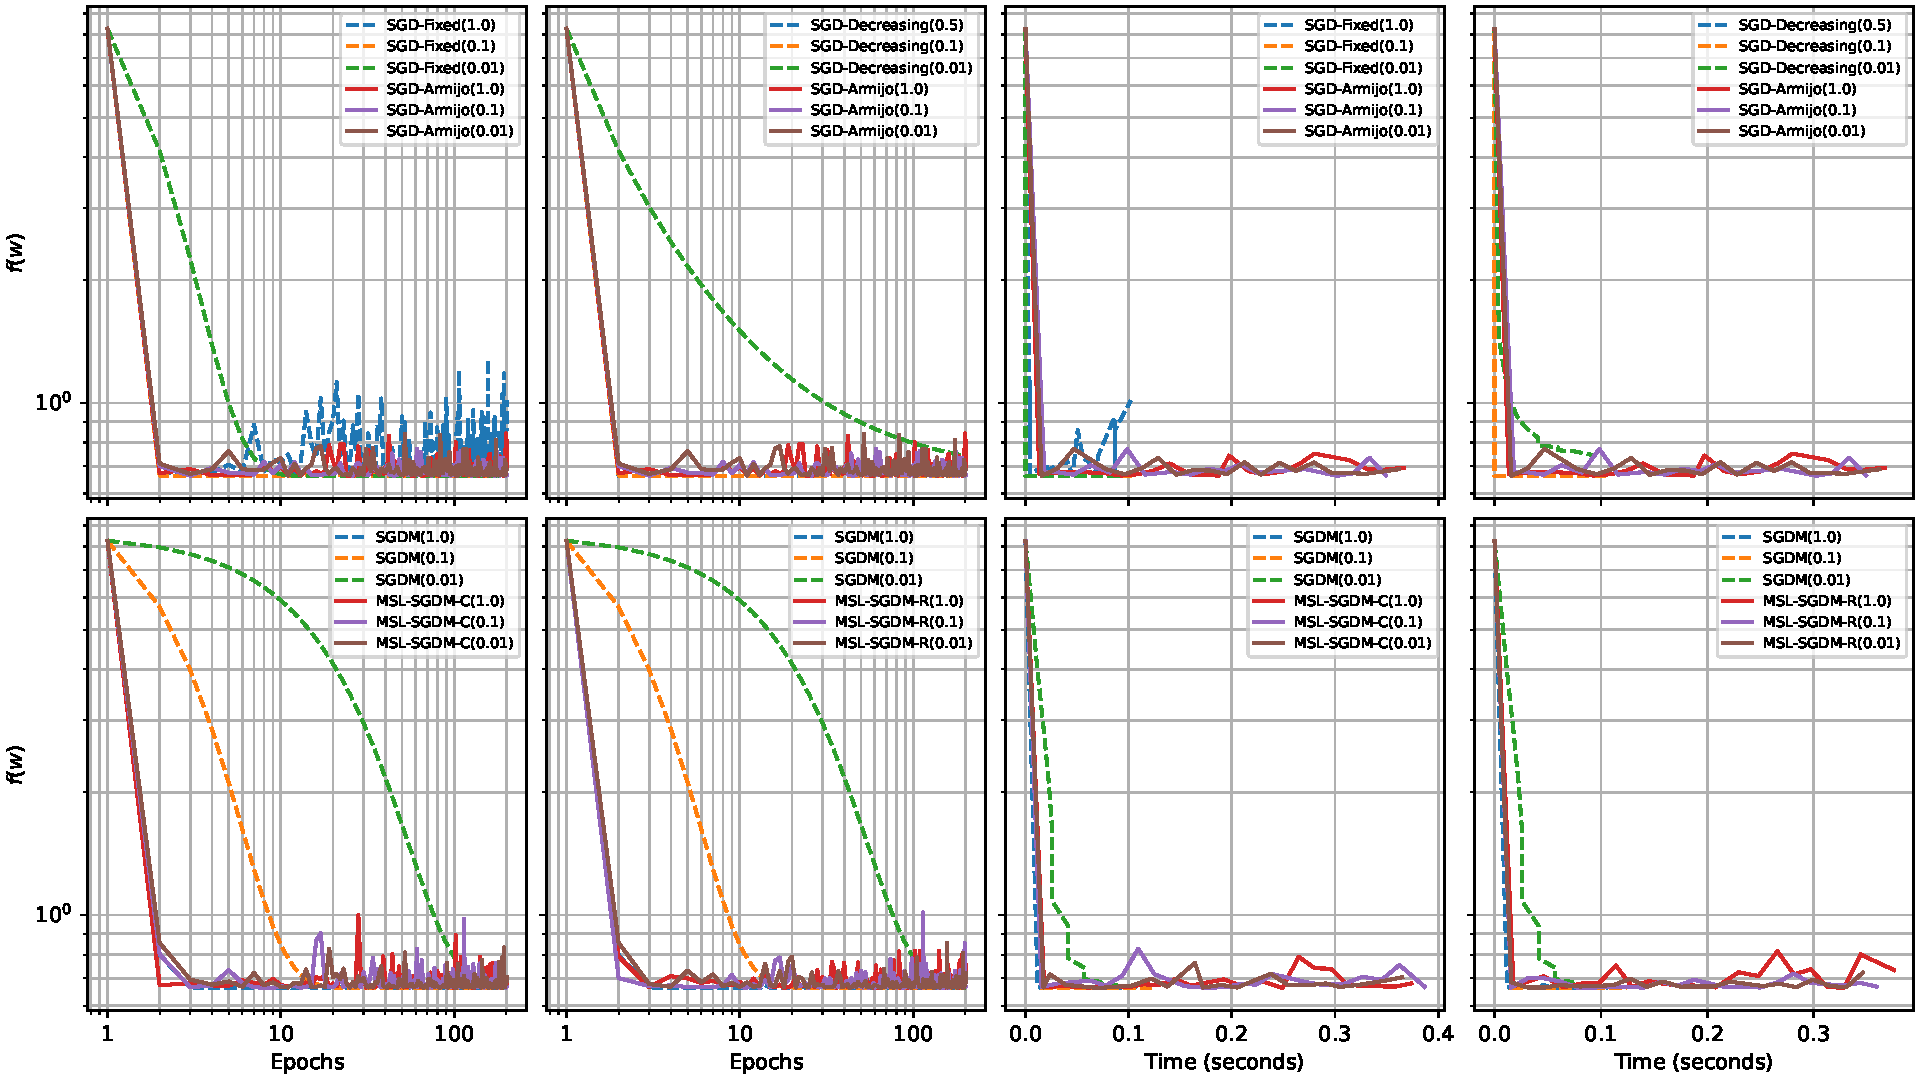
\includegraphics[width=\textwidth]{diab-diagnostic}} \\
% w3a
\subfloat[][\emph{w3a dataset}\label{subfig:w3a-diagnostic}]%
{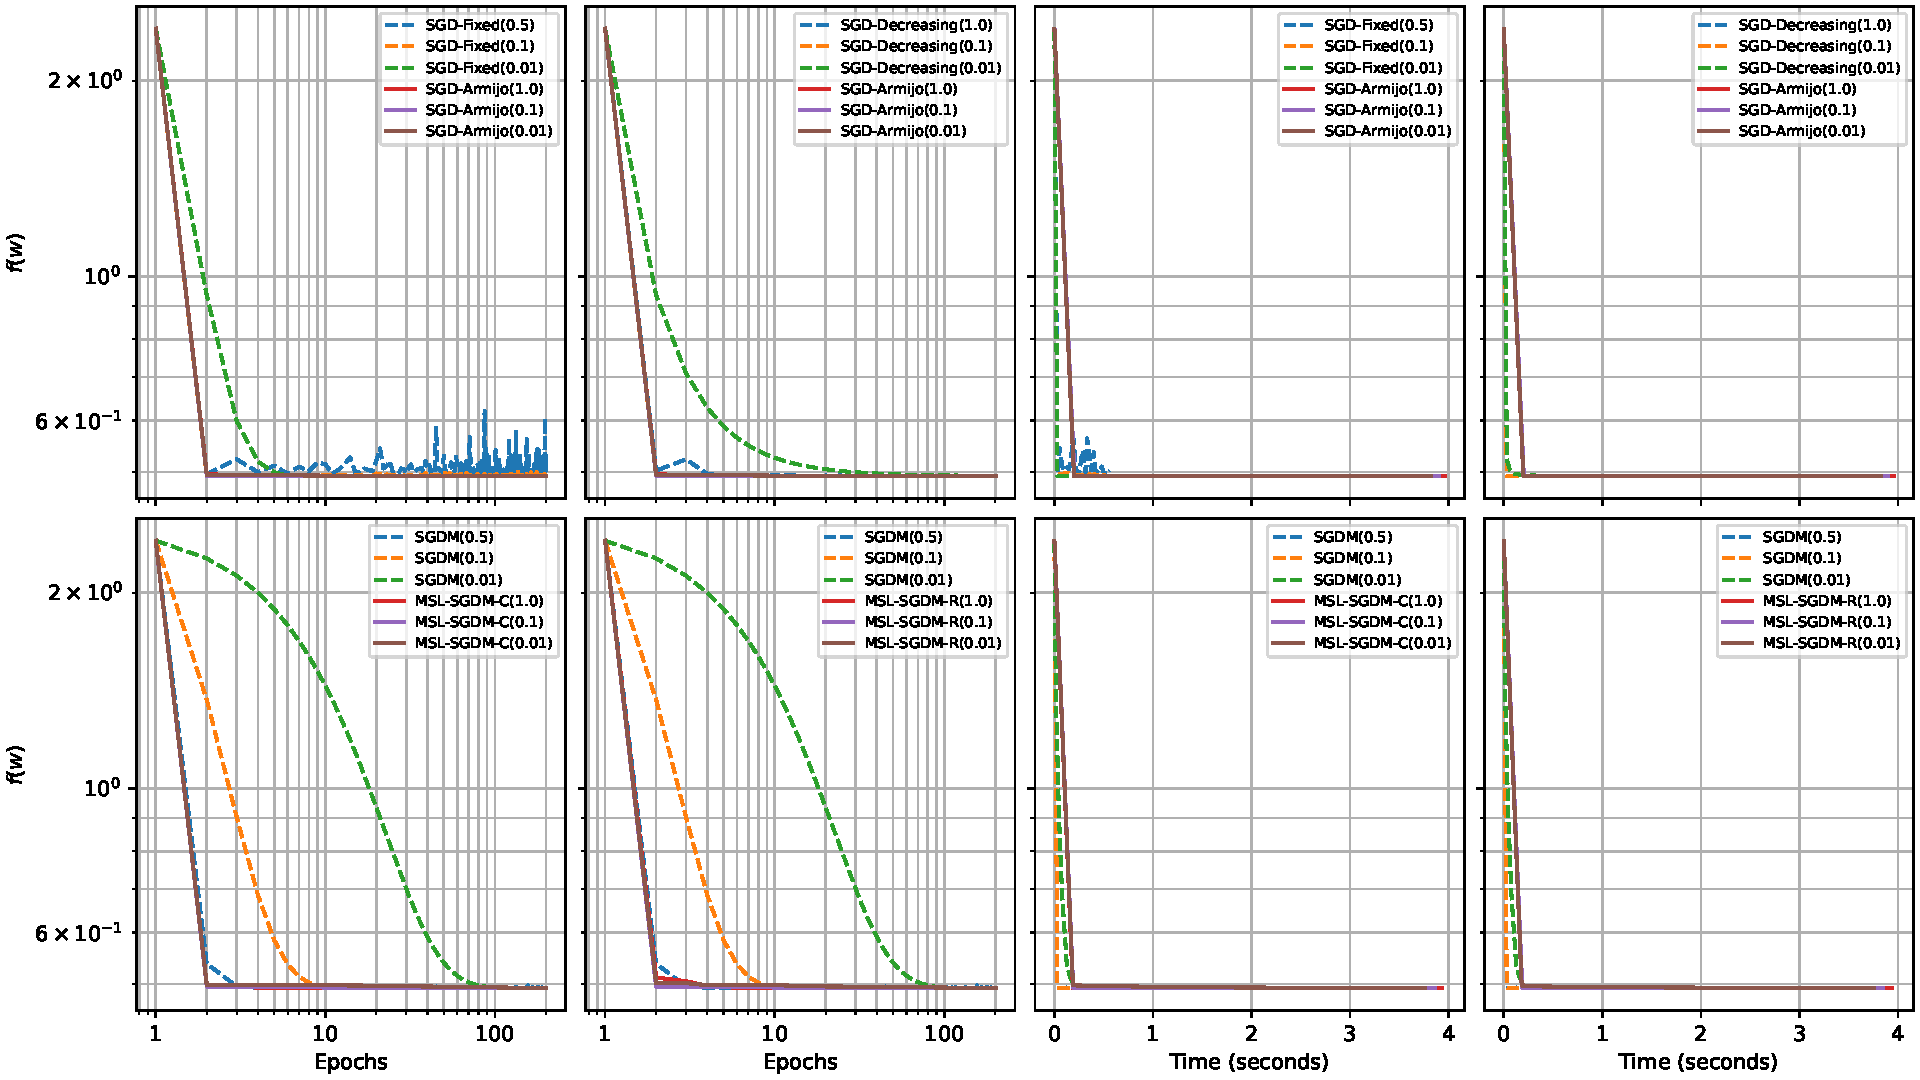
\includegraphics[width=\textwidth]{breast-diagnostic}} \\
\caption[]{w1a and w3ar}
\label{fig:diab-breast}
\end{figure}

\begin{figure}
\centering
% Phishing
\subfloat[][\emph{Phishing dataset}\label{subfig:phish-diagnostic}]%
{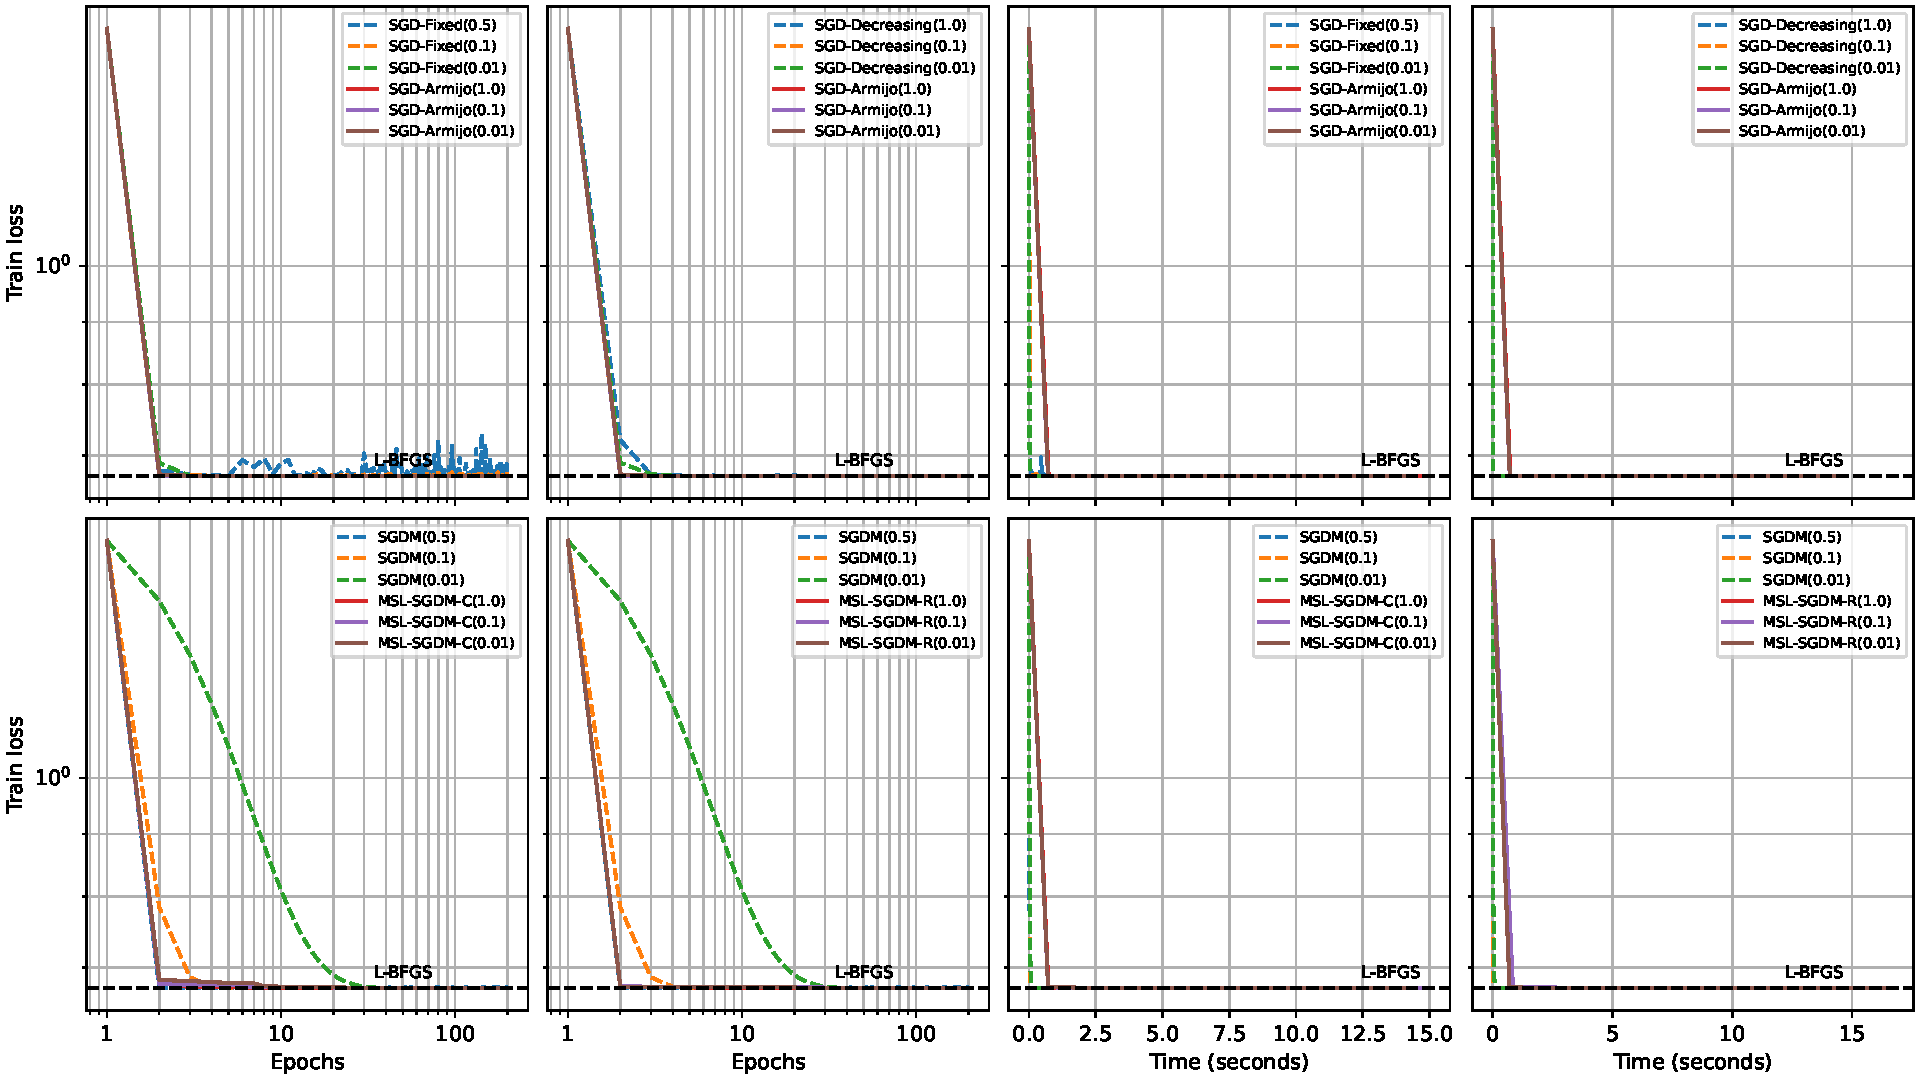
\includegraphics[width=\textwidth]{svm-diagnostic}} \\
% a2a
\subfloat[][\emph{a2a dataset}\label{subfig:a2a-diagnostic}]%
{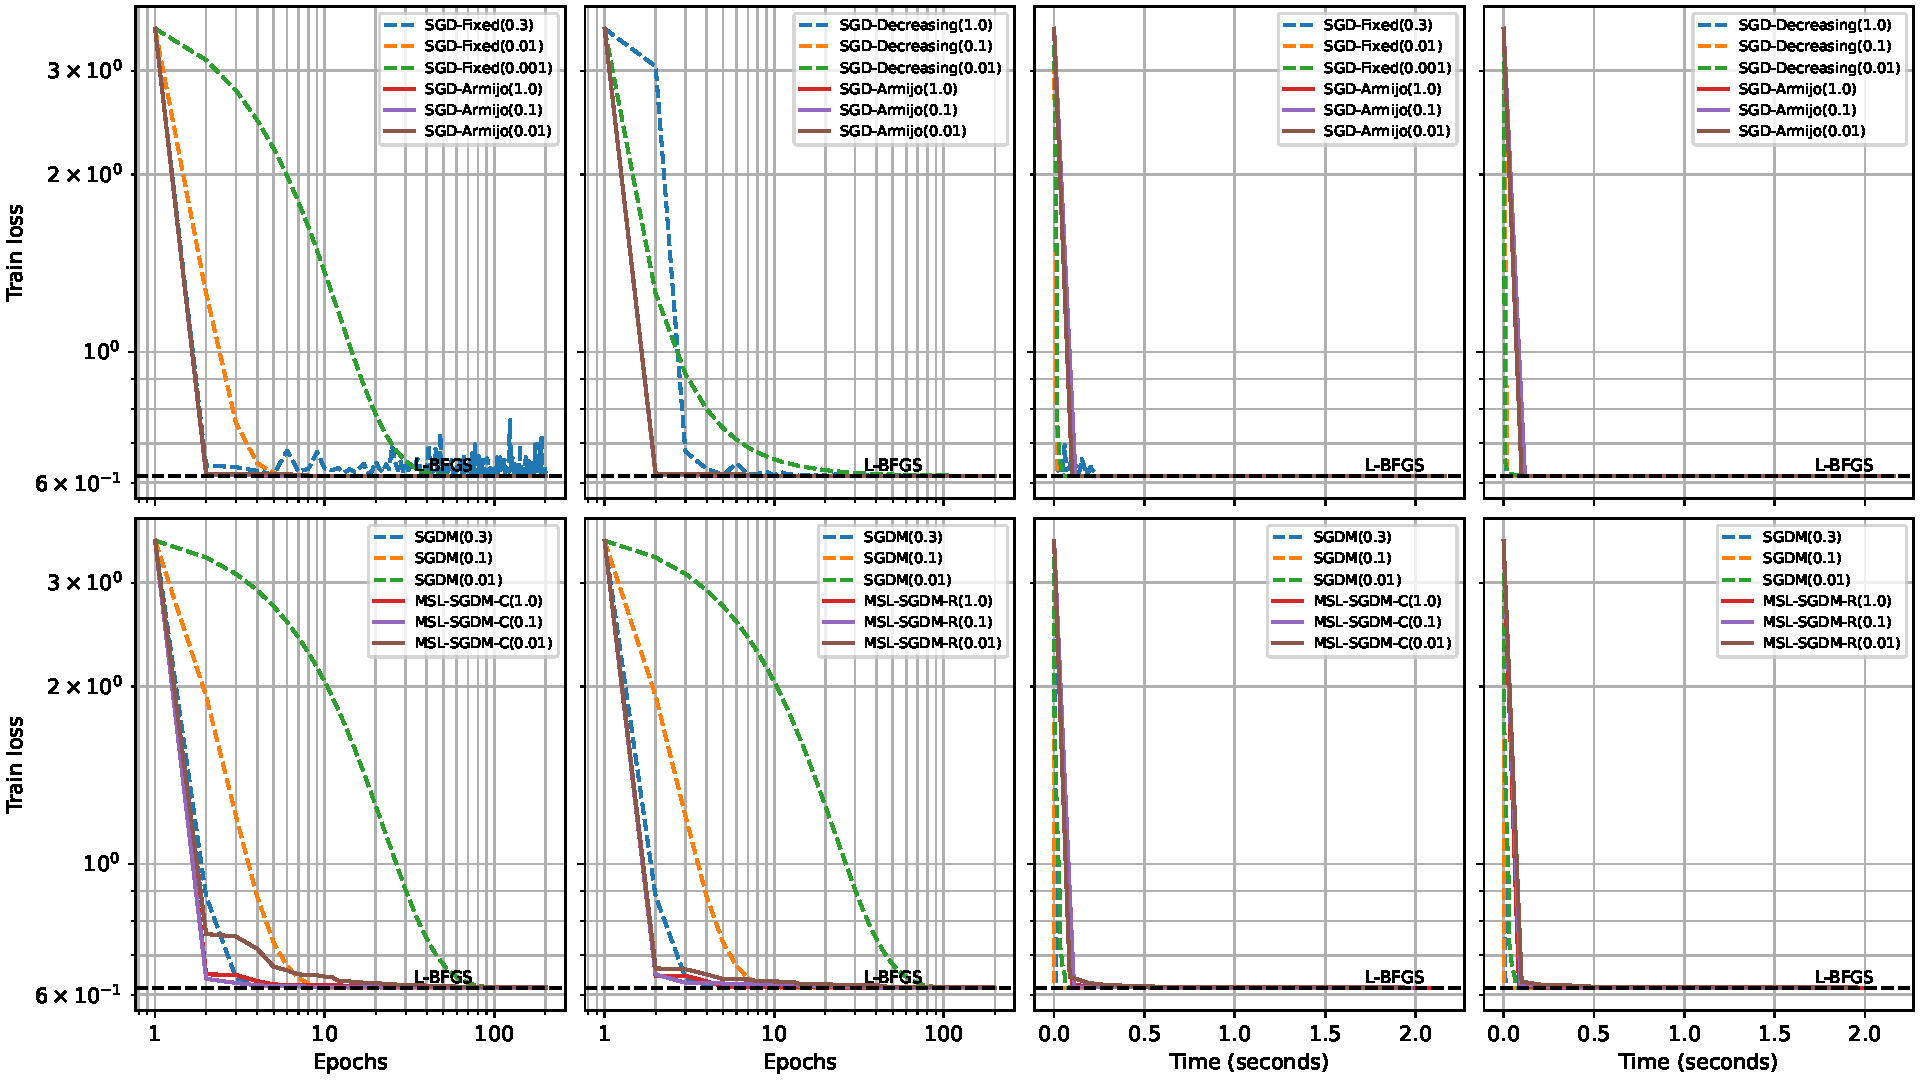
\includegraphics[width=\textwidth]{austr-diagnostic}}
\caption[]{Phishing and a2a datasets}
\label{fig:phish-austr}
\end{figure}

\begin{figure}
\centering
% mushrooms
\subfloat[][\emph{Mushrooms dataset}\label{subfig:mush-diagnostic}]%
{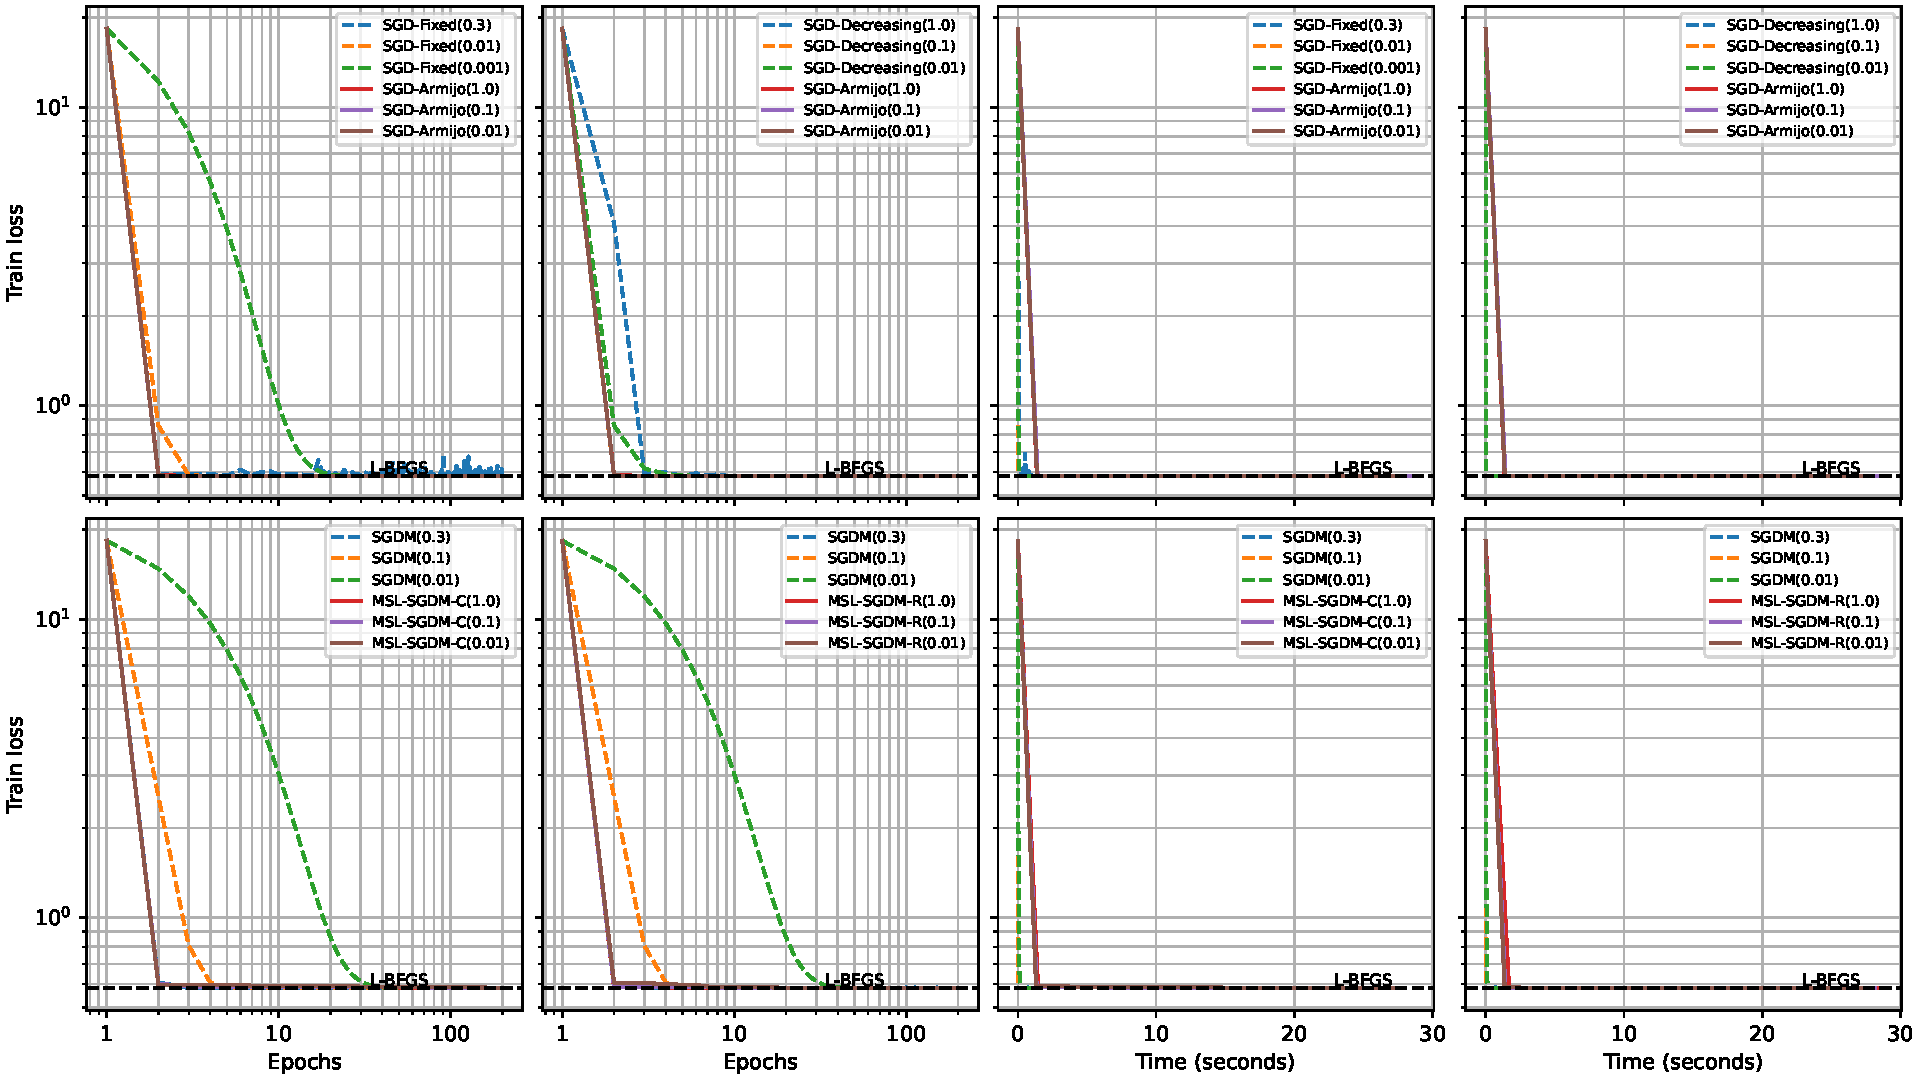
\includegraphics[width=\textwidth]{mush-diagnostic}} \\
% german
\subfloat[][\emph{German dataset}\label{subfig:german-diagnostic}]%
{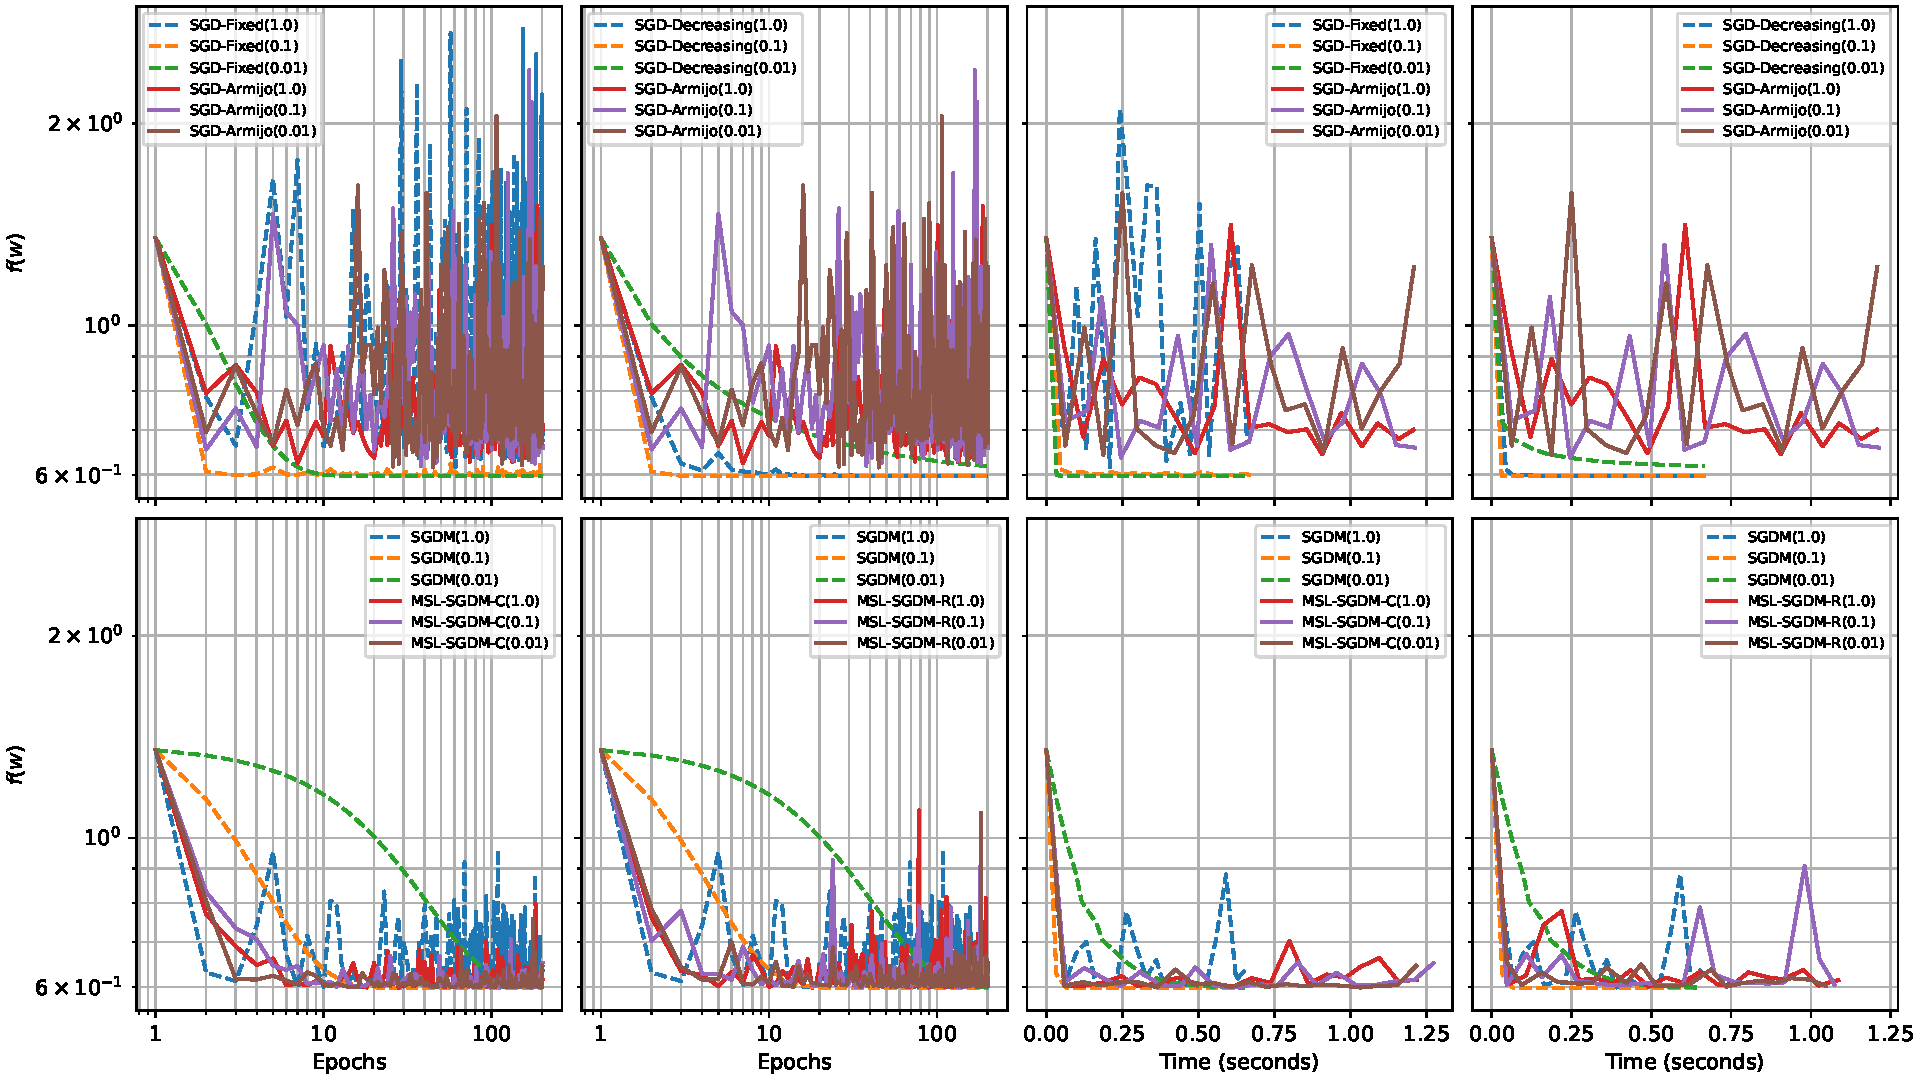
\includegraphics[width=\textwidth]{german-diagnostic}}
\caption[]{Mushrooms and German datasets}
\label{fig:mush-german}
\end{figure}

%\cleardoublepage
% ***************************************************** %
%\section{Mathematical background}
% ***************************************************** %

%\begin{defs}[Convex function]\label{def:conv_fun}
%	Let $S\subseteq\R^n$ be a convex set, a function $f\colon S\to\R$ is said to be convex if the hessian matrix is semi-positive-defined. If the hessian matrix is positive-defined, then the function is strictly convex.
%\end{defs}
%
%\begin{thm}[Weirstrass theorem]\label{thm:weirs}
%	Let $f\colon\R^n\to\R$ be a continuous function and $S\subseteq\R^n$ a compact set. Then function $f$ admits global minimum in $S$.
%\end{thm}
%
%\begin{cor}[Sufficient condition]\label{cor:weirs1}
%	If function $f\colon\R^n\to\R$ is a continuous and coercive function, then $f$ admits global minimum in $\R^n$.
%\end{cor}
%
%\begin{prop}[Coercivity of a quadratic function]
%	A quadratic function $\func(x)=\frac{1}{2}x^TQx-c^Tx$ is said to be coercive if and only if the symmetric matrix $Q\in\R^{n\times n}$ is positive-defined.
%\end{prop}
%
%\begin{prop}[Unique global minimum]\label{prop:min_unique}
%	Let $S\subseteq\R^n$ be a convex set, let $f\colon S\to\R$ be a strictly convex function. Then the global minimum, if exists, is unique.
%\end{prop}
%
%\begin{prop}[First order optimality condition]
%	$\bar{x}$ is a local minimum for $f\colon\R^n\to\R$ of class $f\in C^1(\R^n)$ if and only if $\nabla\func(\bar{x})=0$.
%\end{prop}
%
%\begin{prop}[Second order optimality condition]\label{prop:opt_second}
%	$\bar{x}\in\R^n$ is a local minimum for $f\colon\R^n\to\R$ of class $f\in C^2(\R^n)$ if and only if
%	\[\nabla\func(\bar{x})=0\quad\wedge\quad \nabla^2\func(\bar{x})\,\,\,\text{positive semi-definite}\]
%\end{prop}

% add definition of coercive function and proposition about compact sets?
% add gradient descent?
